% Template file for a standard thesis
\documentclass[11pt,notitlepage]{isuthesis}
% notitlepage is used because \begin{abstract} uses titlepage by default, which resets the page numbers

\usepackage[pdftex]{graphicx}
% Standard, old-style thesis
\usepackage{isutraditional}   
\chaptertitle
% Old-style, thesis numbering down to subsubsection
\alternate
\usepackage{rotating}
% Bibliography without numbers or labels
\usepackage{natbib}
\usepackage{chapterbib}
%\renewcommand\bibsection{\section*{\ref name}}
%\renewcommand\bibsection{\section*}
\renewcommand{\bibsection}{\section{References}}


\bibliographystyle{apa}  % changed from apa, abbrv, unsrtnat
%\includeonly{titletoc,chapter1}
%Optional Package to add PDF bookmarks and hypertext links
\usepackage[pdftex,hypertexnames=false,linktocpage=true]{hyperref}
\hypersetup{colorlinks=true,linkcolor=blue,anchorcolor=blue,citecolor=blue,filecolor=blue,urlcolor=blue,bookmarksnumbered=true,pdfview=FitB}

%\usepackage{titletoc}
\usepackage{hyperref}



\overfullrule=0pt
%%%%%%%%%%%%%%%%%%%%%

% The following piece of code removes extra space on the top of each chapter
%  that is default of latex report class documents

\usepackage{etoolbox}
\makeatletter
\patchcmd{\@makechapterhead}{50\p@}{0pt}{}{}
\patchcmd{\@makeschapterhead}{50\p@}{0pt}{}{}
\makeatother

%%%%%%%%%%%%%%%%%%%%%%%
%%%%%%%%%%%%%%%%%%%%%%%%%
% Removing Bold characters in the Table of Contents
% % Alternatively to this the isuthesis.cls file has been changed by default in the
% % line section \renewcommand{\l@chapter}[2]{\addpenalty{-\@highpenalty}....
%\titlecontents{chapter}
%[0pt]                                               % left margin
%{}%
%{\contentsmargin{0pt}                               % numbered entry format
%    \thecontentslabel\enspace%
%    \large}
%{\contentsmargin{0pt}\large}                        % unnumbered entry format
%{\titlerule*[.5pc]{.}\contentspage}                 % filler-page format (e.g dots)
%[]                                                  % below code (e.g vertical space)
%%%%%%%%%%%%%%%%%%%%%%%%%%

%%%%%%%%%%%%%%%%%%%%%%%%%%%%%%%
% In order to change space between the Table of contents items go to isuthesis.cls
% line  \renewcommand{\l@chapter}[2]{\addpenalty{-\@highpenalty}....
% change \vkip values

%%%%%%%%%%%%%%%%%%%%%%%%%%
%% This is to minimize orphan lines. Might not be possible to entirely remove them
% Method 1 of doing this
\widowpenalty100000
\clubpenalty100000

% Method 2 of doing this
\usepackage[all]{nowidow}
%%%%%%%%%%%%%%%%%%%%%%%%%%%

%%% control bibliography spacings
% \newlength{\bibitemsep}\setlength{\bibitemsep}{\baselineskip}
% % plus .05\baselineskip minus .05\baselineskip}
% \newlength{\bibparskip}\setlength{\bibparskip}{0pt}
% \let\oldthebibliography\thebibliography
% \renewcommand\thebibliography[1]{%
%   \oldthebibliography{#1}%
%   \setlength{\parskip}{\bibitemsep}%
%   \setlength{\itemsep}{\bibparskip}%
% }
% \usepackage{setspace}
% \setlength{\bibsep}{2sp}


%%%%%%%%%%%%%%%%%%%%%%%%%%%%%%%%%%
% %% aligning lof captions
% \usepackage{tocloft}

%%%%%%%%%%%%%%%%%%%%%%%%%%%%%%%%%%
%% Set the margins in the whole document
\geometry{letterpaper, left=1in, top=1in, right=1in, bottom=1in, includehead=true} 
%%%%%%%%%%%%%%%%%%%%%%%%%%%%%%%%%%

\begin{document}
\DeclareGraphicsExtensions{.jpg,.pdf,.mps,.png}
%\begin{singlespace}
\def\@makechapterheada{\vspace*{-2cm}\titlepage} % in order to reduce the space between margin and heading in titlepage
% Template Titlepage File
\@makechapterheada\titlepage  % using definition from thesis.tex reduce the space between margin and heading in titlepage
\title{This is the title of a thesis
submitted to Iowa State University\\
Note that only the first letter of
the first word and proper names
are capitalized}
\author{Wilbur Terrance Johnson}
\degree{MASTER OF SCIENCE}
%\major{Human Development and Family Studies (Marriage and Family Therapy)}
\comajors{Statistics; Computer Science}{}

\level{master's}
%\mprof{Susan D. Ross}
% In case of co majors please comment out the mprof line above and use the following two lines of mprofs and cmprofs to defines the two co-major profs
\mprofs{ABC}
\cmprofs{DEF}

\members{Mary Jones \\ Bjork Petersen \\}
\disclaimertitlepage{The student author, whose presentation of the scholarship herein was approved by the program of study committee, is solely responsible for the content of this dissertation/thesis. The Graduate College will ensure this dissertation/thesis is globally accessible and will not permit alterations after a degree is conferred.}
%{The student author and the program of study committee are solely responsible for the content of this dissertation/thesis. The Graduate College will ensure this dissertation/thesis is globally accessible and will not permit alterations after a degree is conferred.}

\notice

% Add these additional lines for a Doctoral Dissertation
%\degree{DOCTOR OF PHILOSOPHY}
%\level{doctoral}
%\format{dissertation}
%\committee{4}
%\members{Mary Jones \\ Bjork Petersen \\ Sam Anders \\ Harold Jones}
% Add these additional lines for a Creative Component
% - also comment out the \maketitle command
%\format{Creative Component}
%\submit{the graduate faculty}
\maketitle

%\end{singlespace}
% Optional thesis dedication
\chapter*{DEDICATION}

I would like to dedicate this thesis to my wife Glenda and
to my daughter Alice without whose support I would not have
been able to complete this work.
I would also like to thank my friends and family for their loving guidance and
financial assistance during the writing of this work.


% Table of Contents, List of Tables and List of Figures
{
\pdfbookmark[1]{TABLE OF CONTENTS}{table}
\tableofcontents
}
%%%%%%%%%%%%%%%%%%%%%%%%%%%%%%%%%%%%%%%%%
%% The line below adds the word "Page" over the page numbers in TOC, LOT, LOF
\addtocontents{toc}{~\hfill\textbf{Page}\par}
\addtocontents{lot}{~\hfill\textbf{Page}\par}
\addtocontents{lof}{~\hfill\textbf{Page}\par}
%%
\addtocontents{toc}{\def\protect\@chapapp{}} \cleardoublepage \phantomsection
\pagebreak
\addcontentsline{toc}{chapter}{LIST OF TABLES}
%%%%%%%%%%%%%%%%%%%%%%%%%%%%%%%%%%%%%%%%%
\listoftables
\cleardoublepage \phantomsection \addcontentsline{toc}{chapter}{LIST OF FIGURES}
%%%%%%%%%%%%%%%%%%%%%%%%%%%%%%%%%%%%%%%%%
\listoffigures


% Comment out the next line if NOT using chaptertitle
\addtocontents{toc}{\def\protect\@chapapp{CHAPTER\ }}
%Optional Acknowledgements
\cleardoublepage \phantomsection
\specialchapt{ACKNOWLEDGMENTS}

I would like to take this opportunity to express my thanks to those
who helped me with various aspects of conducting research and the writing
of this thesis.
First and foremost, Dr. Susan D. Ross for her guidance, patience and support
throughout this research and the writing of this thesis.
Her insights and words of encouragement have often inspired me and renewed
my hopes for completing my graduate education.
I would also like to thank my committee members for their efforts
and contributions to this work: Dr. August Tanner and
Dr. Lewis Hargrave.
I would additionally like to thank
Dr. Tanner for his guidance throughout the initial stages of my
graduate career and Dr. Hargrave for his inspirational teaching style.

%Optional thesis abstract
\cleardoublepage \phantomsection
\specialchapt{ABSTRACT}

This is the text of my abstract that is part of the thesis itself.
The abstract describes the work in general and the heading and style
match the rest of the document.

\newpage
\pagenumbering{arabic}

% Chapter 1 of the Thesis Template File
\chapter{INTRODUCTION}
This chapter will have the introduction to your thesis as a whole.

This is the opening paragraph to my thesis which
explains in general terms the concepts and hypothesis
which will be used in my thesis.

With more general information given here than really
necessary.

\section{Overview}

Here initial concepts and conditions are explained and
several hypothesis are mentioned in brief.

\subsection{Hypothesis}

Here one particular hypothesis is explained in depth
and is examined in the light of current literature.

\subsubsection{Parts of the hypothesis}

Here one particular part of the hypothesis that is 
currently being explained is examined and particular
elements of that part are given careful scrutiny.

% Below \subsubsection
% Sectional commands: \paragraph and \subparagraph may also be used

\subsection{Second Hypothesis}

Here one particular hypothesis is explained in depth
and is examined in the light of current literature.

\subsubsection{Parts of the second hypothesis}

Here one particular part of the hypothesis that is 
currently being explained is examined and particular
elements of that part are given careful scrutiny
\cite{allen}, \cite{bruner}, \cite{prime-number-theorem} abcd.

\section{Criteria Review}

Here certain criteria are explained thus eventually
leading to a foregone conclusion.


% \section{Bibliography}
\bibliographystyle{apa}
% \vspace{-20pt}
\begingroup
    \setlength{\bibsep}{13.2pt}
    \linespread{1}\selectfont
    \bibliography{master_bib}
\endgroup
\clearpage
\pagebreak

\chapter{PAPER 1 TITLE GOES HERE}
\label{polymer_fibers}

\begin{center}
    A paper accepted by \textit{Name of the Journal} \\
    First Author and Second Author
\end{center}

\section{Abstract}
This is the text of my abstract that is part of the thesis itself.
The abstract describes the work in the first paper general. You can use the same abstract as your paper here.

%\pagebreak %remove if needed

% Please include sections as the paper has, some of the following sections are meant as examples of what can be done, the bibliography should be made as given

\section{Overview}

The  construct of this section or any further section is same as the authors paper.
This is the opening paragraph to my thesis which
explains in general terms the concepts and hypothesis
which will be used in my thesis.

With more general information given here than really
necessary.

\section{Introduction}

Here initial concepts and conditions are explained and
several hypothesis are mentioned in brief.

\cite{allen}, \cite{bruner} and \cite{cox}
did the initial work in this area. But in Struss' work [\cite{struss}]
the definitive model is seen.

\subsection{Hypothesis}

Here one particular hypothesis is explained in depth
and is examined in the light of current literature.

\subsubsection{Parts of the hypothesis}

Here one particular part of the hypothesis that is 
currently being explained is examined and particular
elements of that part are given careful scrutiny.

% Below \subsubsection
% Sectional commands: \paragraph and \subparagraph may also be used

\subsection{Second Hypothesis}

Here one particular hypothesis is explained in depth
and is examined in the light of current literature.

\subsubsection{Parts of the second hypothesis}

Here one particular part of the hypothesis that is 
currently being explained is examined and particular
elements of that part are given careful scrutiny.

\section{Criteria Review}

Here certain criteria are explained thus eventually
leading to a foregone conclusion.

\section{Conclusion}\label{conclusion}

The conclusion of the paper goes here.
%\cite{allen}, \cite{bruner} 
\cite{cox}
% \cite{latex} 
\cite{Ancey1996}, \cite{RR73} 
\cite{Aup91}, \cite{Dou72} 

% This section may or may not be included
\section{Appendix: supplemental procedure description}
If there is an appendix that needs to go with the paper it can be as a section

\subsection{Procedure details}
Details of the paper specific appendix procedures


%\section{Bibliography}
\bibliographystyle{apa}
% \vspace{-20pt}
\begingroup
    \setlength{\bibsep}{13.2pt}
    \linespread{1}\selectfont
    \bibliography{master_bib}
\endgroup
\clearpage
\pagebreak
\chapter{PAPER 2 TITLE GOES HERE}
%\label{polymer_fibers}

\begin{center}
    A paper accepted by \textit{Name of the Journal} \\
    First Author and Second Author
\end{center}

\section{Abstract}
This is the text of my abstract that is part of the thesis itself.
The abstract describes the work in the first paper general. You can use the same abstract as your paper here.

%\pagebreak %remove if needed

% Please include sections as the paper has, some of the following sections are meant as examples of what can be done, the bibliography should be made as given

\section{Overview}

The  construct of this section or any further section is same as the authors paper.
This is the opening paragraph to my thesis which
explains in general terms the concepts and hypothesis
which will be used in my thesis.

With more general information given here than really
necessary.

\section{Introduction}

Here initial concepts and conditions are explained and
several hypothesis are mentioned in brief.

\cite{allen}, \cite{bruner} and \cite{cox}
did the initial work in this area. But in Struss' work [\cite{struss}]
the definitive model is seen.

\subsection{Hypothesis}

Here one particular hypothesis is explained in depth
and is examined in the light of current literature.

\subsubsection{Parts of the hypothesis}

Here one particular part of the hypothesis that is 
currently being explained is examined and particular
elements of that part are given careful scrutiny.

% Below \subsubsection
% Sectional commands: \paragraph and \subparagraph may also be used

\subsection{Second Hypothesis}

Here one particular hypothesis is explained in depth
and is examined in the light of current literature.

\subsubsection{Parts of the second hypothesis}

Here one particular part of the hypothesis that is 
currently being explained is examined and particular
elements of that part are given careful scrutiny.

\section{Criteria Review}

Here certain criteria are explained thus eventually
leading to a foregone conclusion.

\section{Conclusion}\label{Conclusion1}

The conclusion of the paper goes here.

\cite{allen}, \cite{bruner}, 
\cite{Hal82},
\cite{Rud73}, \cite{Con90}, 
\cite{Con78}, \cite{KR83}, 
\cite{KR86}

% This section may or may not be included
\section{Appendix: supplemental procedure description}
If there is an appendix that needs to go with the paper it can be as a section

\subsection{Procedure details}
Details of the paper specific appendix procedures

%\section{Bibliography}
\bibliographystyle{apa}
% \vspace{-20pt}
\begingroup
    \setlength{\bibsep}{13.2pt}
    \linespread{1}\selectfont
    \bibliography{master_bib}
\endgroup
\clearpage
\pagebreak
\chapter{PAPER 3 TITLE GOES HERE}
%\label{polymer_fibers}

\begin{center}
    A paper accepted by \textit{Name of the Journal} \\
    First Author and Second Author
\end{center}

\section{Abstract}
This is the text of my abstract that is part of the thesis itself.
The abstract describes the work in the first paper general. You can use the same abstract as your paper here.

%\pagebreak %remove if needed

% Please include sections as the paper has, some of the following sections are meant as examples of what can be done, the bibliography should be made as given

\section{Methods and procedures}

This is the opening paragraph to my thesis which
explains in general terms the concepts and hypothesis
which will be used in my thesis.

With more general information given here than really
necessary.

\section{Introduction}

Here initial concepts and conditions are explained and
several hypothesis are mentioned in brief.

As can be seen in Table~\ref{nothing} it is truly
obvious what I am saying is true.

\begin{table}[h!tb] \centering
\isucaption{This table shows a standard empty table}
\label{nothing}

\vspace{ 2 in}
\end{table}

\subsection{Hypothesis}

Here one particular hypothesis is explained in depth
and is examined in the light of current literature.

This can also be seen in Figure~\ref{moon} that the
rest is obvious.

\begin{figure}[h!tb] \centering

\vspace{ 2 in}
\isucaption{This table shows a standard empty figure}
\label{moon}
\end{figure}

\subsubsection{Parts of the hypothesis}

Here one particular part of the hypothesis that is 
currently being explained is examined and particular
elements of that part are given careful scrutiny.

% Below \subsubsection
% Sectional commands: \paragraph and \subparagraph may also be used

\subsection{Second Hypothesis}

Here one particular hypothesis is explained in depth
and is examined in the light of current literature.

\subsubsection{Parts of the second hypothesis}

Here one particular part of the hypothesis that is 
currently being explained is examined and particular
elements of that part are given careful scrutiny.

%\addtocontents{toc}{\protect\newpage} % Adds \newpage in "\tableofcontents"
\section{Criteria Review}

Here certain criteria are explained thus eventually
leading to a foregone conclusion as can be seen in
Table~\ref{nevermore}.

\begin{table}[h!tb] \centering
\setlength{\captionwidth}{3.5 in}
\isucaption{This table shows a standard empty table with a limited caption width}
\label{nevermore}

\vspace{ 2 in}
\end{table}

\section{Results}
Include any results

\section{Conclusion}\label{conclusion2}

The conclusion of the paper goes here.

%\cite{allen}, \cite{bruner} 
\cite{Rea85}
\cite{Enf87}, \cite{Dau75} 
\cite{KPS75}

% This section may or may not be included
\section{Appendix: supplemental procedure description}
If there is an appendix that needs to go with the paper it can be as a section

\subsection{Procedure details}
Details of the paper specific appendix procedures


% \section{Bibliography}
\bibliographystyle{apa}
% \vspace{-20pt}
\begingroup
    \setlength{\bibsep}{13.2pt}
    \linespread{1}\selectfont
    \bibliography{master_bib}
\endgroup
\clearpage
\pagebreak
\chapter{PAPER 4 TITLE GOES HERE}
% \label{polymer_fibers1}

\begin{center}
    A paper accepted by \textit{Name of the Journal} \\
    First Author and Second Author
\end{center}

\section{Abstract}
This is the text of my abstract that is part of the thesis itself.
The abstract describes the work in the first paper general. You can use the same abstract as your paper here.

%\pagebreak %remove if needed

% Please include sections as the paper has, some of the following sections are meant as examples of what can be done, the bibliography should be made as given
%\section{Overview}

This is the opening paragraph to my thesis which
explains in general terms the concepts and hypothesis
which will be used in my thesis.

With more general information given here than really
necessary.

\section{Introduction}

Here initial concepts and conditions are explained and
several hypothesis are mentioned in brief.

Of course, data on this as seen in Table~\ref{data}
is few and far between.

\begin{table}[h!tb] \centering
\isucaption{Moon Data}
\label{data}
% Use: \begin{tabular{|lcc|} to put table in a box
\begin{tabular}{lcc} \hline
\textbf{Element} & \textbf{Control} & \textbf{Experimental} \\ \hline
Moon Rings & 1.23 & 3.38 \\
Moon Tides & 2.26 & 3.12 \\
Moon Walk & 3.33 & 9.29 \\ \hline
\end{tabular}
\end{table}


\subsection{Hypothesis}

Here one particular hypothesis is explained in depth
and is examined in the light of current literature.

Or graphically as seen in Figure~\ref{mgraph}
it is certain that my hypothesis is true.

\begin{figure}[h!tb] \centering

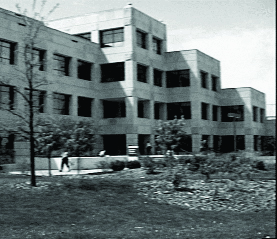
\includegraphics{Images/dc5}

\isucaption{Durham Centre}
\label{mgraph}
\end{figure}

\subsubsection{Parts of the hypothesis}

Here one particular part of the hypothesis that is 
currently being explained is examined and particular
elements of that part are given careful scrutiny.

% Below \subsubsection
% Sectional commands: \paragraph and \subparagraph may also be used

\subsection{Second Hypothesis}

Here one particular hypothesis is explained in depth
and is examined in the light of current literature.

\subsubsection{Parts of the second hypothesis}

Here one particular part of the hypothesis that is 
currently being explained is examined and particular
elements of that part are given careful scrutiny.

\section{Criteria Review}

Here certain criteria are explained thus eventually
leading to a foregone conclusion.

\section{Results}

\section{Conclusion}\label{conclusion3}

The conclusion of the paper goes here.

% This section may or may not be included
\section{Appendix: supplemental procedure description}
If there is an appendix that needs to go with the paper it can be as a section

\subsection{Procedure details}
Details of the paper specific appendix procedures

%\cite{allen}, \cite{bruner} 
\cite{Rad87}
\cite{MOR91}, \cite{Lom73} 
\cite{Lom91}, \cite{Lom92} 
\cite{dB59}

% \section{Bibliography}
\bibliographystyle{apa}
% \vspace{-20pt}
\begingroup
    \setlength{\bibsep}{13.2pt}
    \linespread{1}\selectfont
    \bibliography{master_bib}
\endgroup
\clearpage
\pagebreak
\chapter{FUTURE WORK SUMMARY AND DISCUSSION}
\label{future-work}


This is the opening paragraph to my thesis which
explains in general terms the concepts and hypothesis
which will be used in my thesis.

With more general information given here than really
necessary.

\section{SUMMARY AND DISCUSSION}

Here initial concepts and conditions are explained and
several hypothesis are mentioned in brief.


\subsection{Hypothesis}

Here one particular hypothesis is explained in depth
and is examined in the light of current literature.

As can be seen in Table~\ref{nothingelse} it is
truly obvious what I am saying is true.

\begin{sidewaystable} \centering
\isucaption{This table shows almost nothing but is a
sideways table and takes up a whole page by itself}
\label{nothingelse}
% Use: \begin{tabular{|lcc|} to put table in a box
\begin{tabular}{lcc} \hline
\textbf{Element} & \textbf{Control} & \textbf{Experimental} \\ \hline
Moon Rings & 1.23 & 3.38 \\
Moon Tides & 2.26 & 3.12 \\
Moon Walk & 3.33 & 9.29 \\ \hline
\end{tabular}
\end{sidewaystable}

\subsubsection{Parts of the hypothesis}

Here one particular part of the hypothesis that is 
currently being explained is examined and particular
elements of that part are given careful scrutiny. \cite{allen}, \cite{bruner}, \cite{struss}


% Below \subsubsection
% Sectional commands: \paragraph and \subparagraph may also be used


%\section{Criteria Review}

%Here certain criteria are explained thus eventually
%leading to a foregone conclusion.

% \section{Bibliography}

\bibliographystyle{apa}
% \vspace{-20pt}
\begingroup
    \setlength{\bibsep}{13.2pt}
    \linespread{1}\selectfont
    \bibliography{master_bib}
\endgroup
\clearpage
\pagebreak


%%%%%% bibliographies

%\clearpage
%% \nocite{*}
%\unappendixtitle
%\newpage
%% % \phantomsection
%\addcontentsline{toc}{chapter}{BIBLIOGRAPHY}
%\section*{BIBLIOGRAPHY}
%\bibliographystyle{apa}
%\vspace{-20pt}
%\begingroup
%    \setlength{\bibsep}{14.5pt}
%    \linespread{1}\selectfont
%    \bibliography{master_bib}
%\endgroup

% Renders the citations but does not show the bibliography at the end of the thesis
\newsavebox\mytempbib
\savebox\mytempbib{\parbox{\textwidth}{\bibliography{master_bib}}}

\clearpage
\pagebreak
% Appendix1 file from standard thesis template

\appendixtitle 
\appendix


%% Use the following two lines for single appendix
%\unappendixtitle
%\singleappendixtitle

% Please note the appendix can be removed if the thesis does not require an overall appendix

\chapter{ADDITIONAL MATERIAL} 
This is now the same as any other chapter except that
all sectioning levels below the chapter level must begin
with the *-form of a sectioning command.

\section*{More stuff}

Supplemental material.

 % Instruction for single appendix look below
% An example second appendix from the example thesis thesis.tex.
\chapter{STATISTICAL RESULTS}

This is now the same as any other chapter except that
all sectioning levels below the chapter level must begin
with the *-form of a sectioning command.

\section*{Supplemental Statistics}

More stuff.

\end{document}